 \documentclass{article}
 \usepackage{graphicx}
 \graphicspath{ {./images/} }
 
 \begin{document}
 
 \begin{center}
     \Huge\textbf{Homework 2: Sukrit Ganesh}\par
 \end{center}
 
  \noindent\makebox[\linewidth]{\rule{\paperwidth}{0.4pt}}\newline
 
 \begin{center}
      \Large\textbf{Problem 1:} Suppose you have a dataset ${x}=\{x_1, x_2, x_3, x_4\}$ consisting of 4 items. You know that $x_1 = 25$ and $x_2 = -15$ and that after standardization, $\hat{x_1} = 0$ and $\hat{x_2} = -1$. \par
 \end{center}
 
 \textbf{Part A: | Find $mean\{x\}$ and $std\{x\}$.}\newline
 
 The following formula standardizes every point in the dataset, where $\mu = mean\{x\}$ and $\sigma = std\{x\}$.
 
 \begin{displaymath}
 \hat{x_i} = \frac{x_i - \mu}{\sigma}  
 \end{displaymath}
 
 We know that $0 = \frac{25 - \mu}{\sigma}$ and $-1 = \frac{-15 - \mu}{\sigma}$ by substituting the given values for $x_1$, $x_2$, $\hat{x_1}$, and $\hat{x_2}$.\newline
 
 We can solve the first equation.
 
 \begin{displaymath}
 0 = \frac{25 - \mu}{\sigma}
 \end{displaymath}
 
 \begin{displaymath}
 0 = 25 - \mu
 \end{displaymath}
 
 \begin{displaymath}
 \mu = 25
 \end{displaymath}
 
 Hence, we find that $mean\{x\} = 25$.\newline
 
 We can substitute $\mu = 25$ into the second equation and subsequently solve for $\sigma$.
 
 \begin{displaymath}
 -1 = \frac{-15 - \mu}{\sigma}
 \end{displaymath}
 
 \begin{displaymath}
 -1 = \frac{-15 - 25}{\sigma}
 \end{displaymath}
 
 \begin{displaymath}
 -1 = \frac{-40}{\sigma}
 \end{displaymath}
 
 \begin{displaymath}
 \sigma = 40
 \end{displaymath}
 
 Hence, we find that $std\{x\} = 40$.\newline
 
 Final Answer: $mean\{x\} = 25$, $std\{x\} = 40$.\newline
 
 \textbf{Part B: | Find $x_3$ and $x_4$ given that $x_3 \leq x_4$.}\newline
 
 Because we already know $mean\{\hat{x}\} = 0$ and $std\{\hat{x}\} = 1$ by definition of a standardized data set, will first find $\hat{x_3}$ and $\hat{x_4}$, then use the standardization formula, $\hat{x_i} = \frac{x_i - \mu}{\sigma}$, where $\mu = mean\{x\}$ and $\sigma = std\{x\}$, to find $x_3$ and $x_4$.\newline
 
 By the definition of the mean, $mean\{\hat{x}\} = \hat{x_1} + \hat{x_2} + \hat{x_3} + \hat{x_4} = 0$ By plugging in $\hat{x_1} = 0$ and $\hat{x_2} = -1$, we get $\hat{x_3} = -\hat{x_4} + 1$.\newline
 
 The formula for standard deviation of a standardized data set is as follows: $\hat{\sigma} = \sqrt{\frac{1}{N}*\sum_{i=0}^{n}((\hat{x_{i}}))^2} = 1$. We can plug in the values $\hat{\sigma}} = 1$, $N = 4$, $\hat{x_1} = 0$, $\hat{x_2} = -1$, and $\hat{x_3} = -\hat{x_4} + 1$ to find $\hat{x_4}$.

 \begin{displaymath}
 1 = \sqrt{\frac{1}{N}*\sum_{i=0}^{n}((\hat{x_{i}})^2}
 \end{displaymath}
 
 \begin{displaymath}
 1 = \sqrt{\frac{1}{N}((\hat{x_{1}})^2+(\hat{x_{2}})^2+(\hat{x_{3}})^2+(\hat{x_{4}})^2)}
 \end{displaymath}
 
 \begin{displaymath}
 1 = \sqrt{\frac{1}{4}((0)^2+(-1)^2+(-\hat{x_{4}}+1)^2+(\hat{x_{4}})^2})
 \end{displaymath}
 
 \begin{displaymath}
 1 = \sqrt{\frac{1}{4}*(1+(-\hat{x_{4}}+1)^2+(\hat{x_{4}})^2})
 \end{displaymath}
 
 \begin{displaymath}
 1 = \frac{1}{4}*(1+(-\hat{x_{4}}+1)^2+(\hat{x_{4}})^2)
 \end{displaymath}
 
 \begin{displaymath}
 3 = (-\hat{x_{4}}+1)^2+(\hat{x_{4}})^2
 \end{displaymath}
 
 \begin{displaymath}
 3 = 2\hat{x_4}^2 - 2\hat{x_4} + 1
 \end{displaymath}
 
 \begin{displaymath}
 0 = 2\hat{x_4}^2 - 2\hat{x_4} - 2
 \end{displaymath}
 
 \begin{displaymath}
 \hat{x_4} = \{1.618, -0.618\}
 \end{displaymath}
 
 Hence, because we know that $\hat{x_3} = -\hat{x_4} + 1$, we find that $\hat{x_3} = -0.618$ when $\hat{x_4} = 1.618$ or $\hat{x_3} = 1.618$ when $\hat{x_4} = -0.618$. However, because $x_3 \leq x_4$, we know that $\hat{x_3} \leq \hat{x_4}$, and that $\hat{x_3} = -0.618$ and $\hat{x_4} = 1.618$.\newline
 
 By rearranging the standardization formula, we get that $x_i = \sigma * \hat{x_i} + mean\{x\}$. Hence, we find that $x_3 = 0.28$ and $x_4 = 89.72$.\newline
 
 Final Answer: $x_3 = 0.28$ and $x_4 = 89.72$. \newline

 \newpage
 
 \noindent\makebox[\linewidth]{\rule{\paperwidth}{0.4pt}}\newline
 
 \begin{center}
      \Large\textbf{Problem 2:} In a population, the correlation coefficient between weight and adiposity is 0.9. The mean weight is 150lb. The standard deviation in weight is 30lb. Adiposity is measured on a scale such that the mean is 0.8, and the standard deviation is 0.1.\par
 \end{center}
 
 \textbf{Part A: | Using this information, predict the expected adiposity of a subject whose weight is 170lb.}\newline
 
 We will use the variables $x$ and $y$ to represent weight and adiposity, respectively. We must first express the given weight in standardized coordinates.\newline
 
 \begin{displaymath}
    \hat{x} = \frac{x - mean\{x\}}{std\{x\}} = \frac{170 - 150}{30} = 0.667
 \end{displaymath}
 
 We then use the correlation coefficient, $r$, to predict $\hat{y}$.
 
 \begin{displaymath}
    \hat{y} = r*\hat{x} = 0.9 * 0.667 = 0.6
 \end{displaymath}
 
 Finally, we use the standardization formula to find $y$ from $\hat{y}$.
 
 \begin{displaymath}
    y = std\{y\}*\hat{y} + mean\{y\} = 0.1 * 0.6 + 0.8 = 0.86
 \end{displaymath}
 
 Hence, we predict that when the weight of a subject is 170lb, the adiposity of that subject is 0.86.\newline
 
 Final Answer: 0.86.\newline
 
 \textbf{Part B: | Using this information, predict the expected weight of a subject whose adiposity is 0.75.}\newline
 
 We must first express the given adiposity in standardized coordinates.\newline
 
 \begin{displaymath}
    \hat{y} = \frac{y - mean\{y\}}{std\{y\}} = \frac{0.75 - 0.8}{0.1} = -0.5
 \end{displaymath}
 
 We then use the correlation coefficient, $r$, to predict $\hat{x}$.
 
 \begin{displaymath}
    \hat{x} = r*\hat{y} = 0.9 * -0.5 = -0.45
 \end{displaymath}
 
 Finally, we use the standardization formula to find $x$ from $\hat{x}$.
 
 \begin{displaymath}
    x = std\{x\}*\hat{x} + mean\{x\} = 30 * -0.45 + 150 = 136.5
 \end{displaymath}
 
 Hence, we predict that when the adiposity of a subject is 0.75, the weight of that subject is 136.5 lbs.\newline
 
 Final Answer: 136.5 lbs.\newline
 
 \textbf{Part C: | How reliable do you expect this prediction to be? Why? (your answer should be a property of correlation, not an opinion
about adiposity or weight)}\newline
 
 The correlation coefficient, 0.9, is very close to 1. Coefficients closer to 1 indicate a strong correlation, while coefficients closer to 0 indicate a weak (or nonexistant) correlation. The high correlation coefficient makes the data prediction more likely to be near the actual value. Generally, statisticians use +- 0.8 as the lowest absolute value of the correlation coefficient to indicate significant correlation, and the correlation coefficient between weight and adiposity certainly falls above that threshold. \newline
 
 \newpage

 \begin{center}
      \Large\textbf{Problem 3:} In a population, the correlation coefficient between family income and child IQ is 0.30. The mean family income was \$60,000. The standard deviation in income is \$20,000. IQ is measured on a scale such that the mean is 100, and the standard deviation is 15.\par
 \end{center}

 \textbf{Part A: | Using this information, predict the expected IQ of a child whose family income is \$70,000.}\newline
 
 We will use the variable $x$ to represent income and the variable $y$ to represent IQ. We must first express the given income in standardized coordinates.\newline
 
 \begin{displaymath}
    \hat{x} = \frac{x - mean\{x\}}{std\{x\}} = \frac{70000 - 60000}{20000} = 0.5
 \end{displaymath}
 
 We then use the correlation coefficient, $r$, to predict $\hat{x}$.
 
 \begin{displaymath}
    \hat{y} = r*\hat{x} = 0.3 * 0.5 = 0.15 
 \end{displaymath}
 
 Finally, we use the standardization formula to find $y$ from $\hat{y}$.
 
 \begin{displaymath}
    y = std\{y\}*\hat{y} + mean\{y\} = 0.15 * 15 + 100 = 102.25
 \end{displaymath}
 
 Hence, we predict that when the family income of a subject is \$70,000, that subject's IQ is 102.25.\newline
 
 Final Answer: 102.25.\newline
 
 \textbf{Part B: | How reliable do you expect this prediction to be? Why? (your answer should be a property of correlation, not an opinion
about IQ)}\newline
 
 The correlation coefficient of 0.3 falls far below the threshold of 0.8, which most stasticians agree is the minimum correlation coefficient which indicates significant correlation. The closer the correlation coefficient gets to 0, the weaker the correlation gets. The correlation coefficient of 0.3 is quite close to 0 and quite insignificant, and most statisticians would not consider the two variables to be correlated. \newline
 
 \textbf{Part C: |The family income now rises — does the correlation predict that the child will have a higher IQ? Why?}\newline
 
 Because the correlation coefficient, 0.3, is positive, an increase in family income correlates with an increase in IQ. However, the correlation coefficient is so low that most statisticians would not consider the two variables to be significantly correlated. Although the correlation is very weak, it is positive, meaning that children who grow up in households with a higher family income will tend to have higher IQs. \newline
 
 \newpage
 
 \begin{center}
      \Large\textbf{Problem 4:} At http://lib.stat.cmu.edu/DASL/Datafiles/cigcancerdat.html, you will find a dataset recording per capita cigarette sales and cancer deaths per 100 K population for a variety of cancers, recorded for 43 states and the District of Columbia in 1960.\par
 \end{center}

 \textbf{Part A: | Plot a scatter plot of lung cancer deaths against cigarette sales, using the two letter abbreviation for each state as a marker. You should see two fairly obvious outliers. The backstory at http://lib.stat.cmu.edu/DASL/Stories/cigcancer.html suggests that the unusual sales in Nevada are generated by tourism (tourists go home, and die there) and the unusual sales in DC are generated by commuting workers (who also die at home).}\newline
 
 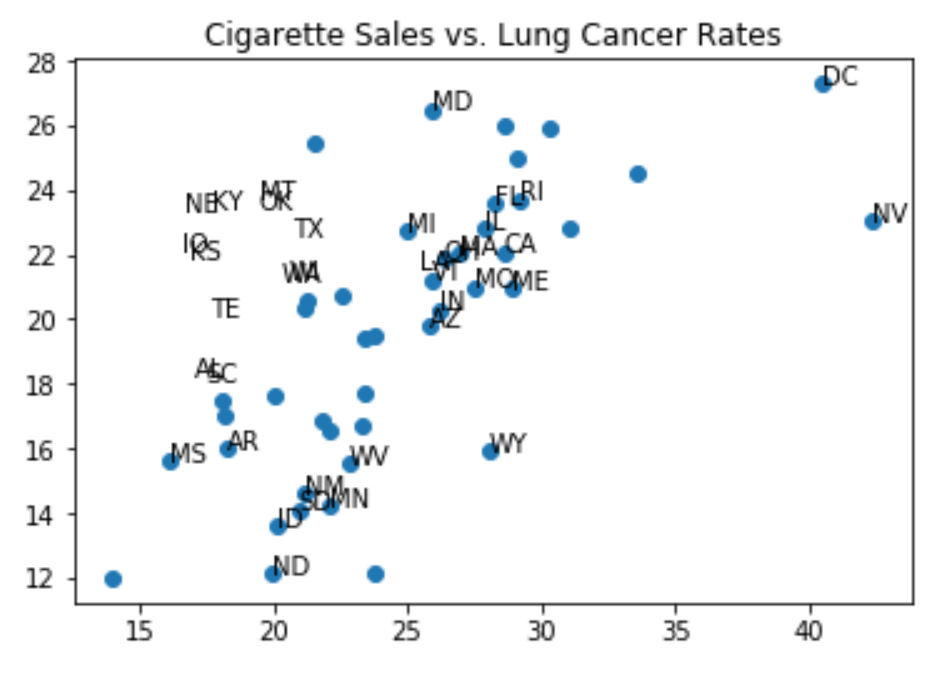
\includegraphics{HW2_1.PNG}
 
 \textbf{Part B: | What is the correlation coefficient between per capita cigarette sales and lung cancer deaths per 100 K population? Compute this with, and without the outliers. What effect did the outliers have? Why?}\newline
 
 The correlation coefficient with outliers is 0.697 (using pearson correlation function from scipy). The correlation coefficient without outliers is 0.714. Because the two outliers do not "align" well with the correlation (in other words, the difference between the prediction and actual value of an outlier is high), removing outliers increases the correlation coefficient since a larger portion of the data points will generally fit with the correlation.\newline
 
 Final Answer: 0.697 with outliers, 0.714 without outliers.\newline
 
 \textbf{Part C: | What is the correlation coefficient between per capita cigarette sales and bladder cancer deaths per 100 K population? Compute this with, and without the outliers. What effect did the outliers have? Why?}\newline
 
 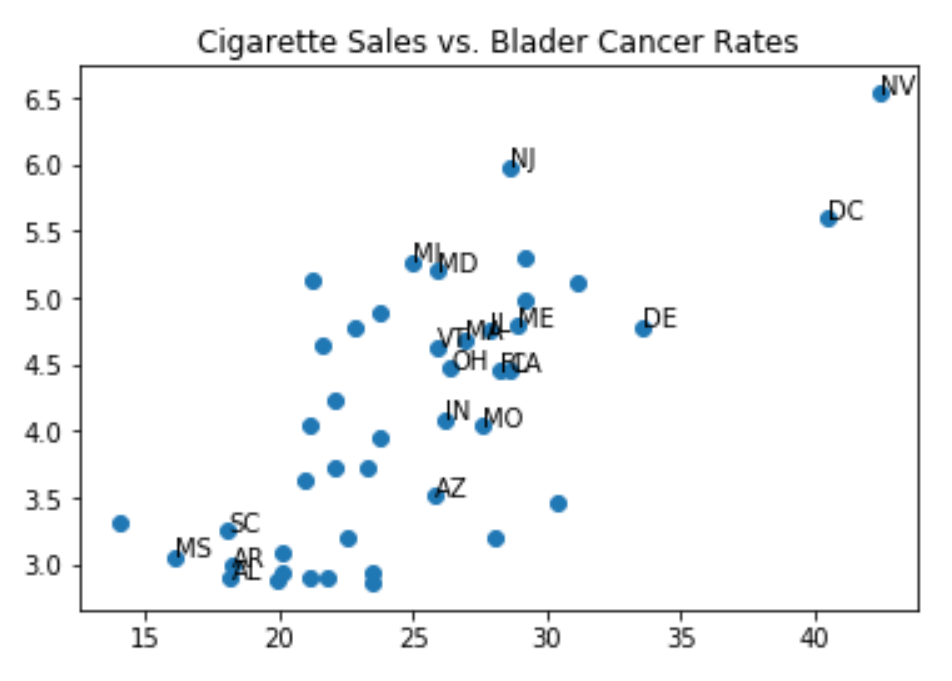
\includegraphics{HW2_2.PNG}
 
 The correlation coefficients are 0.704 and 0.709 with and without outliers, respectively. In this case, Nevada and D.C. were both kept, because they lay near the regression line. However, New Jersey, which lays quite far from the regression line, was removed as an outlier. Once again, the removal of the outlier increased the correlation coefficient.\newline
 
 Final Answer: 0.704 with outliers, 0.709 without outliers.\newline
 
 \textbf{Part D: | What is the correlation coefficient between per capita cigarette sales and kidney cancer deaths per 100 K population? Compute this with, and without the outliers. What effect did the outliers have? Why?}\newline
  
 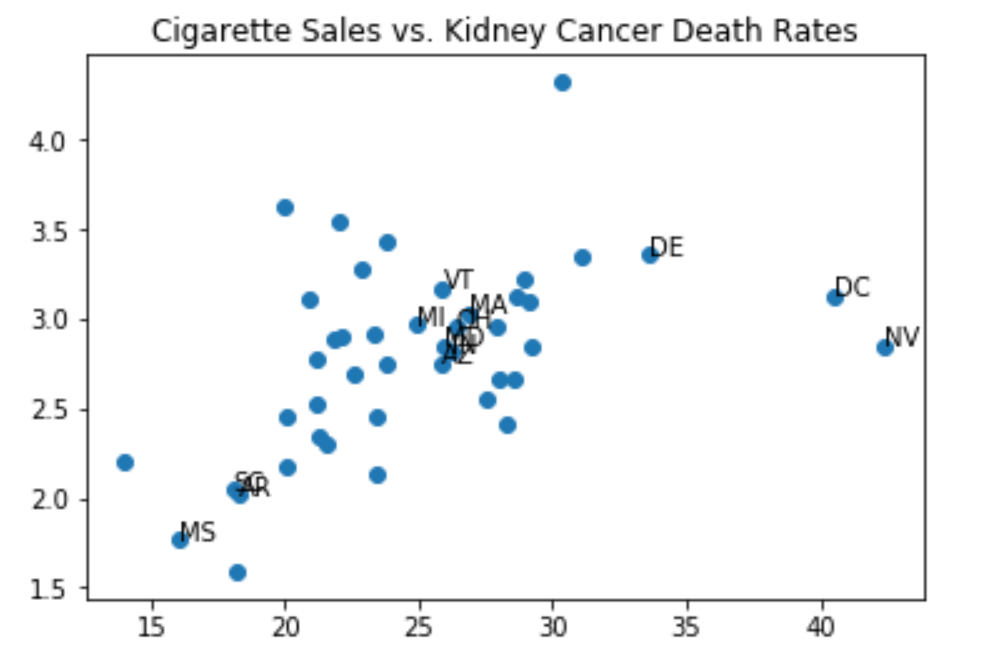
\includegraphics{HW2_3.PNG}

 The correlation coefficients are 0.487 and 0.580 with and without outliers, respectively. In this case, Nevada and D.C. were both removed because they were located far away from the cluster of data and far off the regression line. As in part b, the removal of the outliers, increased the correlation coefficient.\newline
 
 Final Answer: 0.487 with outliers, 0.580 without outliers.\newline
 
 \textbf{Part E: | What is the correlation coefficient between per capita cigarette sales and leukemia deaths per 100 K population? Compute this with, and without the outliers. What effect did the outliers have? Why?}\newline
  
 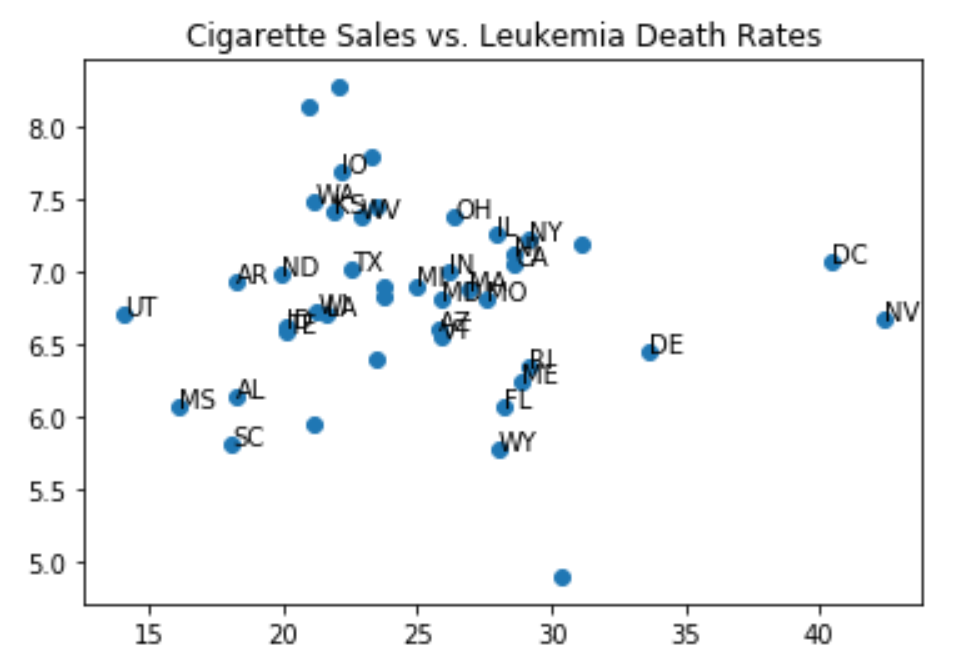
\includegraphics{HW2_4.PNG}

 The correlation coefficients are -0.068 and -0.101 with and without outliers, respectively. In this case, Nevada and D.C. were both classified as outliers because they lay far from the cluster of data and farthest from the regression line. As in part b, the removal of the outliers, which did not fit well with the correlation and lay far away from most of the data points, increased the correlation coefficient's magnitude (which means the correlation became stronger). Interestingly, the correlation between the two variables is negative, indicating that lower cigarette sales correlate with higher leukemia death rates. \newline
 
 Final Answer: -0.068 with outliers, -0.101 without outliers.\newline
 
 \textbf{Part F: | You should have computed a positive correlation between cigarette sales and lung cancer deaths. Does this mean that smoking causes lung cancer? Why?}\newline
  
 Even though it is widely agreed that smoking causes cancer, the data does not definitively prove a causation. One of the most common misconceptions in statistics is that correlation automatically means causation. Such an assumption is unfounded. A correlation between two sets of data merely states how one variable will change when an other changes, not whether that variable CAUSES the other variable to change. In this case, higher cigarette sales correlate with higher rates of lung cancer, but there is no proof directly linking smoking to cigarette deaths in this graph. For example, the amount of cake eaten may positively correlate with higher median income, but this may be due to the fact that people in developed countries tend to eat more cake due to more disposable income and access to premium goods, not because eating cake miraculously increases your earnings. Furthermore, cigarette sales and smoking are actually two different variables; it is certainly possible that cigarettes are not being smoked in the same state they are bought. Overall, the graph does not definitely prove that smoking causes lung cancer. \newline
 
 \textbf{Part G: | You should have computed a negative correlation between cigarette sales and leukemia deaths. Does this mean that smoking cures leukemia? Why?}\newline
  
 The assumption that smoking cures leukemia is nonsensical. First off, the correlation coefficient between cigarette sales and leukemia deaths was -0.101 without outliers, indicating an extremely weak correlation. A correlation coefficient with such a low magnitude is virtually insignificant. Furthermore, correlation does not mean causation. Just because one variable tends to change in a certain way when another variable changes doesn't mean that a change in one variable causes a change in another variable. Like part g, a confounding variable may cause the negative correlation. For instance, urban residents may overall consume more cigarettes but also have better access to leukemia treatment since hospitals are usually located in cities, resulting in states with higher urban populations having both more leukemia deaths and cigarette sales (I don't know if this is true or not, but you get the point). Correlation is not equal to causation, and just because two variables are correlated does not mean that a change in one variable causes a change in another variable. \newline
 
 \newpage
 
 \begin{center}
     \Large\textbf{Problem 5:} Download the daily adjusted closing stock prices for current year of the Coca-Cola Company (KO) and PepsiCo (PEP).\par
 \end{center}
 
 \textbf{Part A: | Use this data to find the correlation coefficient between  the stock prices of these two corporations.}\newline\newline
 
 The correlation coefficient between the closing stock prices of PepsiCo and Coca-Cola is 0.894.\newline
 
 Final answer: 0.894\newline
 
 \textbf{Part B: | Plot a scatter plot with KO prices on the horizontal axis and PEP prices on the vertical axis.}\newline\newline
 
 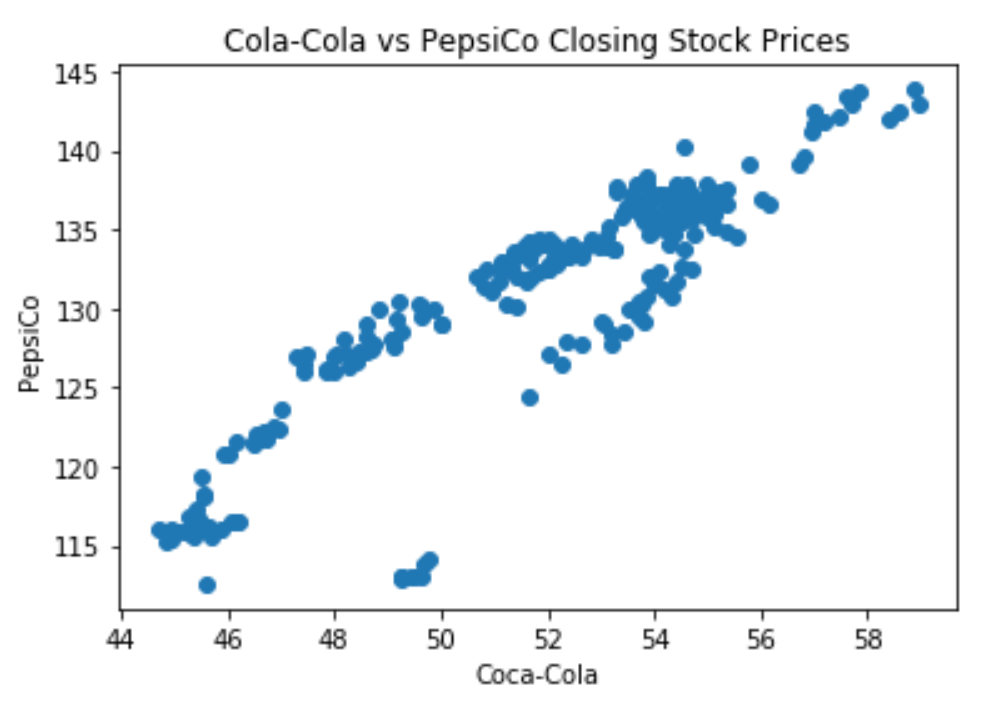
\includegraphics{HW2_5.PNG}
 
 \textbf{Part C: | Add a prediction line to your plot that shows predictions of PEP prices from KO prices.}\newline\newline
 
 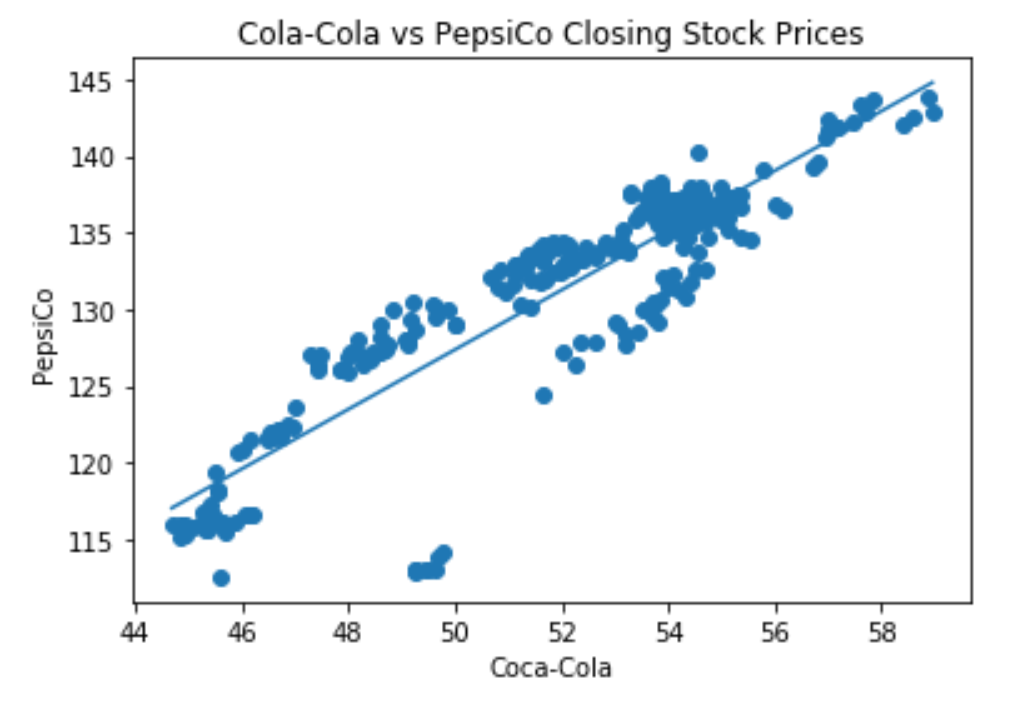
\includegraphics{HW2_6.PNG}
 
 \newpage
 
 \begin{center}
     \Large\textbf{Problem 6:} Let {$\hat{x_i}$} be the standardized data set that is derived from {$x_i$} and has $N$ items. Prove the vector $\langle \frac{\hat{x_1}}{\sqrt{N}}, \frac{\hat{x_2}}{\sqrt{N}}, ... , \frac{\hat{x_N}}{\sqrt{N}} \rangle$ has unit length.\par
 \end{center}
 
 We will prove that the magnitude of the vector $\langle \frac{\hat{x_1}}{\sqrt{N}}, \frac{\hat{x_2}}{\sqrt{N}}, ... , \frac{\hat{x_N}}{\sqrt{N}} \rangle$ is 1. We can express the magnitude of of the vector as the following:
 
 \begin{equation}
    magnitude = \sqrt{(\frac{\hat{x_1}}{\sqrt{N}})^2 + (\frac{\hat{x_2}}{\sqrt{N}})^2 + ... + (\frac{\hat{x_N}}{\sqrt{N}})^2} 
 \end{equation}
 
 \begin{equation}
     = \sqrt{\sum_{i=0}^{N}\frac{(\hat{x_i}^2)}{N}}
 \end{equation}
 
 \begin{equation}
     = \sqrt{\frac{1}{N}*\sum_{i=0}^{N}(\hat{x_i})^2}
 \end{equation}
 
 Recall that the formula for standard deviation is the following:
 
 \begin{displaymath}
     \hat{\sigma} = \sqrt{\frac{1}{N}*\sum_{i=0}^{n}((\hat{x_{i}}-mean\{\hat{x}\}))^2}
 \end{displaymath}
 
  Because the data set is standardized, we know that the standard deviation equals 1 and the mean equals 0. By plugging in the values 1 and 0 for mean and standard deviation, respectively, we get the following equation:
 
 \begin{equation}
    \sqrt{\frac{1}{N}*\sum_{i=0}^{N}(\hat{x_i})^2} = 1
 \end{equation}
 
 Because the left side of equation (4) is the same as the right side of equation (3), we prove that the magnitude of the vector is equal to 1.\newline
 
 \begin{center}
     Q.E.D. :)
 \end{center}
 
 \end{document}

